\documentclass[oribibl]{llncs2e/llncs}
\usepackage{geometry}                % See geometry.pdf to learn the layout options. There are lots.
\geometry{letterpaper}                   % ... or a4paper or a5paper or ... 
\usepackage{graphicx}
\usepackage{tabularx}
%\usepackage{multicolumn}
\usepackage{color}
\graphicspath{{WarpTask/figures/}{Res/figures/}} %do not forget the / at the end

\title{VLI - a library for high precision integer and polynomial arithemtic}
\author{Timoth\'ee Ewart\inst{1}\thanks{Acknowledgments: Maxim Milakov, Peter Messmer:   NVIDIA,   Williams Sawyer, Gilles Fourestey:  CSCS, HP2C funding, hp2c.ch}  , Andreas Hehn$^2$, Matthias Troyer\inst{2} and Thierry Giamarchi\inst{1}}

\institute{Universit\'e de Gen\`eve, \email{timothee.ewart@gmail.com}  \and Eidgen\"ossische Technische Hochschule Z\"urich }

\begin{document}
\maketitle


%%%%%%%%%%%%%%%%%%%%%%%%%%%%%%%%%%%%%%%%%%%%%%%%%%%%%%%%%%%%%%%%%%%%%%%%%%%%%%%
\begin{abstract}
We present a high-performance C++ library for high but fixed precision
(128 to 512 bit) integer arithmetic and symbolic polynomial
computations. While the large integer and polynomial computation parts
of the library can be used independently optimized kernels for symbolic
polynomials with large integer coefficients are provided. The kernels
were manually optimized in assembly language for the x86-64 and power64
architectures. Our main target application is high-temperature series
expansions which require inner products of large vectors of polynomials
with large integer coefficients. For this purpose we implemented a
tunable hybrid CPU/GPU inner product function using OpenMP and NVIDIA
CUDA with inline PTX assembly. This way we make optimal use of today's
and upcoming hybrid supercomputers and attain $65\%$ of the peak
performance of the current NVIDIA Kepler GPU. Compared to a pure CPU
solution using the GNU Multiple Precision Arithmetic Library (GMP) we
gain a speedup of 10x for a pure CPU inner product and 60x using a GPU
accelerator.
\end{abstract}
%%%%%%%%%%%%%%%%%%%%%%%%%%%%%%%%%%%%%%%%%%%%%%%%%%%%%%%%%%%%%%%%%%%%%%%%%%%%%%%

\section{Introduction}
\begin{itemize}
\item {\bf Why did we develop the library?}
\item Applications of large integers and polynomials in many fields of science, e.g.\ cryptography
\item our intention: special purpose library for high-temperature series expansions.
\item HTSE require symbolic polynomials with arbitrary precise coefficients. Coefficients can be represented as integers.
\item maximal integer size known beforehand
\item Hot spot of HTSE inner products of vectors of such polynomials.
\item {\bf Problems with existing libraries:}
\item GMP integers \cite{GMP} are dynamic in size and optimized to cover a large range of large integers up to several thousand bits. We need only up to 512 bits.
\item inner products of polynomials are well suited for GPUs $\rightarrow$ specialized GPU kernels required.
\end{itemize}


%%%%%%%%%%%%%%%%%%%%%%%%%%%%%%%%%%%%%%%%%%%%%%%%%%%%%%%%%%%%%%%%%%%%%%%%%%%%%%%

\section{Large integers}
\begin{itemize}
\item {\bf Description:}
\item signed integer arithmetic
\item fixed size (128-512bit)
\item all standard integer operations (arithmetic, comparison and bit operations)
\item in addition to that: multiply-add, extended multiplication which doubles the number of bits, extended add which increases the size by one 64bit word.
\item {\bf Implementation details:}
\item data is stored as 64 bit integer arrays.
\item two-complement representation
\item stack based $\rightarrow$ cheap memory allocation
\item addition and multiplication using the standard schoolbook algorithms.
\item Numbers are two small for Toom\cite{Toom} or FFT based approaches like the Sch\"onhage-Strassen algorithm\cite{Schonhage}.
\item optimized ASM kernels to use hardware features not accessible from C++ (\verb|x86_64| carry addition \verb|adcq|, 64bit multiplication \verb|mulq| which calculates low and hi 64bit part of the result.)
\item TODO which special features do we use on power64?
\item assembly code generated using \verb|BOOST_PP| to compactify the code and minimize bugs.
\end{itemize}

\section{Polynomials}
\begin{itemize}
\item {\bf Description:}
\item symbolic polynomial in 1-4 variables.
\begin{equation}
    p(x,y,z,a) = \sum_{i,j,k,l} c_{ijkl} x^i y^j z^k a^l
\end{equation}
\item either ``dense'' (${i,j,k,l} \le N$) or ``triangular'' ($i+j+k+l \le N$) structure.
\item any arithmetic type as coefficient $c_{ijkl}$
\item addition, subtraction, multiplication with other polynomials and monomials
\item special multiplication which will double the truncation order
\item {\bf Implementation details:}
\item structure and truncation order $N$ is compile time fixed 
\item function hooks to allow custom optimized kernels for certain coefficient types
\item The symbolic variable names are given as template parameter
\item Automatic matching of variable names of different polynomial types using template meta programming.
\end{itemize}

\section{Optimized inner product}
The hot spot of HTSE are inner products of large vectors with symbolic polynomials as components. The coefficients of the polynomials are large integers.
All polynomials are assumed to have the same truncation order.
The inner product will result in a polynomial of twice the order of the original polynomials
with coefficients of twice the width of the original coefficients.
\paragraph{CPU}
\begin{itemize}
\item We use the single large integer kernels
\item OpenMP parallelization: split vectors into chunks, each thread does part of the inner product. Very regular problem, good load balance.
\item A SIMD implementation to perform 4 large integer operations in parallel on current \verb|x86_64| architectures is not useful, since we had to use 32bit integer operations, which increases the number of multiply instructions for a large integer multiplication by a factor of 4 compared to the 64bit based implementation.
Using current Streaming SIMD Extensions (SSE) allows only two 32bit multiplications yielding 64bit results in a SIMD fashion.
Thus a SIMD implementation using SSE will be two times slower than our serial version using 64 bit integers.
We also neglected the carry bit propagation, which needs to be done manually in SSE, while the sequential version takes advantage of the hardware support for carry bit propagation.
\item The upcoming AVX2 will double the vector width and support four 32bit integer multiplications, but no carry bit support.
\end{itemize}
\paragraph{GPU}
\begin{itemize}
\item Many small tasks of the same form. $\rightarrow$ well suited for GPUs.
\item {\bf Implementation details:}
\item based on 32bit integers due to architecture.
\item Element-wise polynomial multiplication + reduction at the end.
\item Each thread calculates one coefficient $c_{IJKL}$ the product polynomial.
\item Several coefficients $a_{ijkl}$, $b_{i'j'k'l'}$ of the polynomials to be multiplied contribute to the same coefficient $c_{IJKL}$
\begin{equation}
    c_{IJKL} = \sum_{i,j,k,l} a_{ijkl} \cdot b_{I-i,J-j,K-k,L-l}
\end{equation}
\item The number of terms in this sum depends on the orders $I,J,K,L$ of the resulting coefficient $\rightarrow$ load inbalance
%\item {\color{blue} We design an execution plan. We group the coefficients of a fictive result polynomial by packet of 32 } into a task and distribute them among the warps of threads (Fig.\ \ref{fig:GPU_load_balance}).
\item Since threads within a warp are executed in a lockstep manner, we try to give all threads within a warp the same amount of work. This way the threads have to wait as little as possible for the other threads of the warp to finish.
\item We group the coefficients by 32 into a ``task'' and distribute them among the warps of threads (Fig.\ \ref{fig:GPU_load_balance}), i.e.\ each thread calculates one coefficient of the resulting polynomial.
\begin{figure}[t]
    \begin{center}
    \mbox{
        \includegraphics[scale=0.37, angle=-90]{coeffs.eps} 
        \includegraphics[scale=0.37, angle=-90]{warp.eps} 
    }
    \caption{Left: Number of contributions to each coefficient of the resulting polynomial (red line) sorted in reverse order and split into tasks. Right: Load balancing of the tasks over the warps.}
    \label{fig:GPU_load_balance}
    \end{center}
\end{figure}
\item {\color{blue} During the execution of a task by a warp,  each threads into the warp get the indices of the fictive coefficient, determine the necessary  contributions and  then calculate the output coefficient}
\item {\color{blue} Reduction is performed under NVIDA standard}
\item {\color{blue} This algorithm is efficient whatever the type of polynomial. But the termination of the contributions of an output coefficient can be tricky}
%\item Coalesced memory access?
\item {\color{blue}  Karatsuba algorithm \cite{Karatsuba1963} for the largest extended multiplication (256 bit to 512 bit) on GPU}
\item Using NVIDIA parallel thread execution (PTX) assembly language to benefit from hardware carry bit propagation \verb|addc.cc| and multiply-add with carry bit propagation \verb|madc.cc|.
\end{itemize}
%%%%%%%%%%%%%%%%%%%%%%%%%%%%%%%%%%%%%%%%%%%%%%%%%%%%%%%%%%%%%%%%%%%%%%%%%%%%%%%

\section{Benchmarks}
\paragraph{Simple integer operations}
\begin{itemize}
\item pure CPU benchmarks were done on a Sandy bridge Intel Xeon E5-2670 with 32 logical cores.
\begin{table}
    \begin{center}
    \begin{tabular}{l|cc|r}
     Operation & Execution & time [s] & Speed-up\\
       & GMP & VLI & \\
     \hline
    \verb|add|, 128 bit & 1.11 & 0.33 & {\bf 3.36x} \\
    \verb|add|, 192 bit & 1.21 & 0.45 & 2.68x \\
    \verb|add|, 256 bit & 1.11 & 0.81 & 1.37x \\
    \verb|add|, 320 bit & 1.25 & 0.81 & 1.54x \\
    \verb|add|, 384 bit & 1.25 & 0.97 & 1.28x \\
    \verb|add|, 448 bit & 1.34 & 1.01 & 1.32x \\
    \verb|add|, 512 bit & 1.31 & 1.07 & {\bf 1.25x} \\
    \hline
    \verb|mul|, 128 bit $\rightarrow$ 256 bit & 1.36 & 0.93 & 1.46x \\
    \verb|mul|, 192 bit $\rightarrow$ 384 bit & 3.21 & 1.18 & {\bf 2.72x} \\
    \verb|mul|, 256 bit $\rightarrow$ 512 bit & 3.74 & 2.04 & 1.83x \\ 
    \end{tabular}
    \caption{Execution time comparison of simple integer operations using the GNU Multiprecision Library and the VLI library for $10^8$ operations.}
    \label{tab:vli_vs_gmp}
    \end{center}
\end{table}
\item Comparing the execution time of simple addition and multiplication operations our implementation for fixed size integers is between $25\%$ and $236\%$ faster for the addition and up to $172\%$ faster for the multiplication (table \ref{tab:vli_vs_gmp}).
\item Note that the reported time is the pure execution time of the operation. All variables were allocated before.
Since our integer library is stack based we do not need expensive calls to \verb|malloc|, which will give an additional speedup for the inner product.
\end{itemize}

\paragraph{Optimized inner product with GPU accelerator}
\begin{itemize}
\item GPU benchmarks were performed on Todi, a Cray XK7 with NVIDIA Tesla K20X GPUs and AMD Opteron CPUs, at the Swiss Center for Scientific Computing (CSCS)
\item Testcase: inner product of two vectors dimension 4096, with ``dense'' and
``triangular'' polynomials of order 1 to 14 with 128 and 256 bit integer
coefficients. Which will result in polynomials of order 2 to 28 with 256 and 512 bit integer coefficiencts, respectively.
\item We estimate the performance in integer operations per second (IOP/s).
\item For the GPU performance estimate we only consider the instructions for the polynomial-polynomial multiplications and neglect the reduction at the end of the inner product.
\begin{figure}[t!]
    \begin{center}
    \mbox{
        \hspace{-0.5cm}
        \includegraphics[scale=0.37, angle=-90]{ME128.eps} 
        \hspace{-0.4cm}
        \includegraphics[scale=0.37, angle=-90]{MC128.eps} 
    }
    \caption{Left: Inner product of dense polynomials with up to 3 variables and 126 to 256 bits coefficients. Right: Inner product of triangular polynomials with up to 3 variables and 126 to 256 bits coefficients.  Size of the vector 4096. For four variables we are limited by the memory of the node. GMP gives similar results whatever the polynomials.}
    \label{ResME}
    \end{center}
\end{figure}

\begin{figure}[t!]
    \begin{center}
    \mbox{
        \hspace{-0.5cm}
        \includegraphics[scale=0.37, angle=-90]{ME128MIPS.eps} 
        \hspace{-0.4cm}
        \includegraphics[scale=0.37, angle=-90]{MC128MIPS.eps} 
        %\hspace{-0.4cm}
        %\includegraphics[scale=0.25, angle=-90]{ME256.eps} 
    }
    \caption{Performance of the inner product of two vectors of dimension 4096 with ``dense'' (left) and ``triangular'' (right) polynomials having 128 bit coefficients on a NVIDIA Tesla K20X (GK110).}
    \label{fig:ResMEMIPS}
    \end{center}
\end{figure}  
\item We reach up to $214$ GIOP/s using 32 bit multiply-add (\verb|madc|)
\item Theoretical maximum for the NVIDIA Tesla K20X is given by Number of Multiprocessors (SMX) $\cdot$ Clock frequency $\cdot$ Instruction throughput of \verb|madc|  =  $14 \, \mathrm{SMX} \cdot 732 \, \mathrm{MHz} \cdot 32 \, \mathrm{ IOP / cycle / SMX} = 327 \, \mathrm{GIOP/s}$. (Multiply-add throughput taken from \cite{CUDAProgramming}).
\item We reach $65\%$ of the peak.
\item Poor performance for low orders as well as for polynomials in 1 symbolic variable, since too little coefficients need to be calculated to saturate the number of available threads (Fig. \ref{fig:ResMEMIPS}).
\item Maximal performance for ``dense'' polynomial in 3 variables with a truncation at 7th order, where we employ $(2\cdot7+1)^3 = 3375$ threads. Using more threads may yield an even better performance, but we start to exceed the size of the texture memory cache and have to load data from the device memory more often, which causes the decrease of performance for higher orders.
\item Polynomials in 4 symbolic variables only up to 6th order due to memory limitations on the device. Could be overcome by splitting the vectors and performing the inner product on these parts sequentially.
\item Performance for ``triangular'' polynomials rises lower with increasing order, because the number of threads used grows slower with the order than for ``dense'' polynomials.
\end{itemize}

%%%%%%%%%%%%%%%%%%%%%%%%%%%%%%%%%%%%%%%%%%%%%%%%%%%%%%%%%%%%%%%%%%%%%%%%%%%%%%%

\section{Conclusion}
\begin{itemize}
\item We presented a C++ library
\item License?
\end{itemize}

%%%%%%%%%%%%%%%%%%%%%%%%%%%%%%%%%%%%%%%%%%%%%%%%%%%%%%%%%%%%%%%%%%%%%%%%%%%%%%%
\bibliographystyle{llncs2e/splncs}
\bibliography{biblio/vlibib}

\end{document}
